%% GBS distribution learning — lab seminar talk
%% Compile with pdflatex (twice). Figures are pulled from ../report/figures/.
\documentclass[10pt,aspectratio=169]{beamer}

\usetheme{Boadilla}
\usecolortheme{seahorse}
\setbeamertemplate{navigation symbols}{}
\setbeamertemplate{caption}[numbered]
\setbeamertemplate{footline}[frame number]

\usepackage[utf8]{inputenc}
\usepackage{amsmath,amssymb,amsfonts,bm}
\usepackage{graphicx}
\usepackage{booktabs}
\graphicspath{{../report/figures/}{figures/}}

% Dirac kets without the physics package (fewer dependencies)
\providecommand{\ket}[1]{\left|#1\right\rangle}
\providecommand{\bra}[1]{\left\langle#1\right|}

\newcommand{\Haf}{\operatorname{Haf}}
\newcommand{\Tor}{\operatorname{Tor}}
\newcommand{\KL}{D_{\mathrm{KL}}}
\newcommand{\nmean}{\bar n}
\newcommand{\vs}{\mathbf{s}}
\newcommand{\vn}{\mathbf{n}}

\title[GBS distribution learning]{Learning Classical Distributions with Gaussian Boson Sampling}
\subtitle{Theory, training, and a chain of improvements}
\author{I.B., L.E.C.E., V.V.P.}
\institute{Lab seminar}
\date{\today}

\begin{document}

\begin{frame}\titlepage\end{frame}

\begin{frame}{Outline}
\tableofcontents
\end{frame}

% ======================================================================
\section{Part I: GBS as a programmable matrix $A$}
% ======================================================================

\begin{frame}{GBS in one equation: program a matrix $A$}
A GBS device is \emph{programmed} by a symmetric $m\times m$ matrix $A$ (the
``graph''). Measuring in the photon-number basis gives, for an outcome
$\vn=(n_1,\dots,n_m)$,
\[
\boxed{\;P_A(\vn)=\frac{1}{Z}\,\frac{\big|\Haf(A_{\vn})\big|^{2}}{n_1!\cdots n_m!}\;},
\qquad A=A^{\mathsf T}\in\mathbb C^{m\times m},\ \ 0\le\lambda_i(A)<1 .
\]
\begin{itemize}
  \item $A_{\vn}$: repeat row/col $i$ exactly $n_i$ times (delete if $n_i=0$);
        $Z$ is the Gaussian normalisation.
  \item {\footnotesize (The physical state lives on a $2m\times2m$ kernel
        $\mathbf A=A\oplus A^\ast$, $Z=\sqrt{\det(I-X\mathbf A)}$ --- see appendix.)}
  \item The device samples configurations $\vn$ with \emph{large}
        $|\Haf(A_{\vn})|^2$ --- why a well-chosen $A$ solves graph problems
        (dense subgraphs, similarity, point processes, chemistry).
\end{itemize}
\begin{block}{Our question}
Can we \emph{train} $A$ so the GBS samples reproduce a prescribed target
distribution? (Unsupervised learning on a GBS device.)
\end{block}
\end{frame}

\begin{frame}{The adjacency matrix $A$}
The $m\times m$ symmetric block $A$ admits a \textbf{Takagi/Autonne decomposition}
\[
A=U\,\mathrm{diag}(\lambda_1,\dots,\lambda_m)\,U^{\mathsf T},\qquad 0\le\lambda_i<1,
\qquad(U\ \text{unitary}),
\]
with the pure-state distribution $P_A(\vn)=\tfrac1Z\,|\Haf(A_{\vn})|^2/\prod_i n_i!$.
\begin{columns}
\begin{column}{0.54\textwidth}
\begin{block}{Hafnian}
\[
\Haf(M)=\!\!\sum_{\mu\in\mathrm{PMP}(2k)}\ \prod_{(i,j)\in\mu}\!M_{ij},
\]
sum over perfect matchings; \#P-hard in general. \alert{$\Haf=0$ for odd
dimension} $\Rightarrow$ contributing $\vn$ have even $\sum_i n_i$ (parity).
\end{block}
\end{column}
\begin{column}{0.46\textwidth}
\begin{block}{Mean photon number}
\[
\nmean=\sum_{i}\frac{\lambda_i^2}{1-\lambda_i^2},
\]
tuned by rescaling $A\to cA$ (\texttt{rescale\_adjacency}). The scale $\nmean$
is a hyperparameter (revisited in Part~II).
\end{block}
\end{column}
\end{columns}
\end{frame}

\begin{frame}{Threshold detectors}
Threshold detectors report only clicks $\vs\in\{0,1\}^m$,
$s_i=\mathbf 1[n_i\ge1]$ (indicator),
i.e.\ they marginalise over all collision configurations with a given support:
\[
P(\vs)=\!\!\sum_{\vn:\,\mathrm{supp}(\vn)=\mathrm{supp}(\vs)}\!\!P_A(\vn)
=\frac{\Tor\!\big(O_{\vs}\big)}{\sqrt{\det\sigma_Q}},\qquad O=I-\sigma_Q^{-1}.
\]
\begin{block}{Torontonian}
\[
\Tor(O)=\sum_{Z\subseteq[k]}\frac{(-1)^{\,k-|Z|}}{\sqrt{\det(I-O_Z)}},
\qquad \text{cost }\sim 2^{k}\ (k=\#\text{clicks}).
\]
\end{block}
This marginalisation (summing collisions into one click) is exactly the source
of the biases we fix in Part~II.
\end{frame}

\begin{frame}{The task: unsupervised learning of a 1-D density}
Target density $p(x)$ on $[x_0,x_1]$, discretised into $K=2^m-2$ bins.
\begin{itemize}
  \item \textbf{Encode} bin $b\mapsto$ click pattern $\vs$ (default: binary of $b$).
  \item Data $\{\vs^{(t)}\}\sim p_{\mathrm{data}}$; fit a GBS model to minimise
  \[
  C(\bm\theta)=\KL\!\big(p_{\mathrm{data}}\,\|\,P_{A(\bm\theta)}\big)
  =\sum_{\vs}p_{\mathrm{data}}(\vs)\,\ln\frac{p_{\mathrm{data}}(\vs)}{P_{A(\bm\theta)}(\vs)} .
  \]
\end{itemize}
\begin{block}{Evaluation}
\emph{Analytic}: compute $P_{A}(\vs)$ for all $2^m$ patterns via the torontonian
(exact, no sampling noise) --- used for all clean numbers.
\emph{Monte Carlo}: sample the device and histogram.
\end{block}
\end{frame}

\begin{frame}{Building the base matrix from data}
Before training we need a base $A$. The baseline (\texttt{A\_from\_samples}):
\emph{put an edge between every pair of clicking modes}.
\[
A_{ij}\ \propto\ \sum_{t}s_i^{(t)}s_j^{(t)}\quad(i\ne j)\qquad\text{(pairwise co-occurrence counts)},
\]
then symmetrise, normalise by $\max_{ij}A_{ij}$, and rescale to the target mean
photon number $\nmean$.
\begin{itemize}
  \item This fixes the model's \textbf{correlation structure}; recall WAW
        afterwards only reweights rows/columns, so it cannot change which modes
        are correlated — only the base $A$ can.
  \item Baseline flaws, fixed in Part~II: self-loops $A_{ii}$ are added only for
        single-click events, and there is \emph{no} parity correction.
\end{itemize}
\end{frame}

\begin{frame}{The WAW parametrization (Banchi--Quesada--Arrazola 2020)}
Keep a fixed base $A$; make the \emph{weights} trainable:
\[
A_W=W\,A\,W,\qquad W=\mathrm{diag}(w_1,\dots,w_m),\qquad
w_k(\bm\theta)=\exp\!\big(-\bm\theta^{\mathsf T}f^{(k)}\big)\in[0,1].
\]
Physicality ($\lambda_i<1$) is preserved for $0\le w_k\le1$. The hafnian
\textbf{factorises}, $\Haf(A_W)=\Haf(A)\det(W)$, so
\[
\boxed{\;P_{A,W}(\vn)=\frac1Z\,\big|\Haf(A_{\vn})\big|^2\prod_{i=1}^m\frac{w_i^{\,n_i}}{n_i!}\;}
\]
--- an exponential family in $\bm\theta$ ($w_i^{n_i}$). In practice the simple
diagonal choice $w_k=e^{\theta_k}$ ($f^{(k)}=\mathbf e_k$) is used.
\end{frame}

\begin{frame}{Training: analytic KL gradient (classical, $O(m)$)}
Because $\Haf(A_{\vn})$ is $\bm\theta$-independent,
\[
\partial_{w_k}P_{A,W}(\vn)=\frac{n_k-\langle n_k\rangle}{w_k}\,P_{A,W}(\vn),\qquad
\langle n_k\rangle=V_{kk}+V_{k+m,k+m}-\tfrac12 .
\]
Hence the KL gradient is pure \textbf{marginal matching}:
\[
\boxed{\;\partial_{\bm\theta}C
=\sum_{k=1}^m\big(\langle n_k\rangle_{\mathrm{GBS}}-\langle n_k\rangle_{\mathrm{data}}\big)\,f^{(k)}\;}
\]
computable in $O(m)$ classically, even when \emph{sampling} is intractable.
\begin{itemize}
  \item Update $\bm\theta\leftarrow\bm\theta-\eta\,\partial_{\bm\theta}C$.
  \item \alert{Only per-mode marginals are matched} $\Rightarrow$ all
        correlations come from the base $A$: the \textbf{initial construction of
        $A$ is decisive} (Part~II).
\end{itemize}
\end{frame}

% ======================================================================
\section{Part II: Improving the pipeline}
% ======================================================================

\begin{frame}{The factorial / parity bias}
Low-squeezing leading term of a $k$-click pattern with support
$S=\mathrm{supp}(\vs)$, $k=|S|$ ($\mathbf 1_S=$ all-ones on $S$):
\[
P(\vs)\approx
\begin{cases}
\big|\Haf(A[\mathbf 1_S])\big|^2, & k\ \text{even},\\[4pt]
\dfrac{1}{2!}\displaystyle\sum_{i^\star\in S}\big|\Haf(A[\mathbf 1_S+e_{i^\star}])\big|^2, & k\ \text{odd}.
\end{cases}
\]
\begin{itemize}
  \item Even $k$: minimal config $\mathbf 1_S$ already has even photon number — no penalty.
  \item Odd $k$: must \emph{double} one mode to reach an even count $\Rightarrow$
        universal $1/2!$ suppression.
\end{itemize}
The naive construction ignores this (and mishandles self-loops) $\Rightarrow$
systematic even/odd imbalance, which WAW (marginals only) cannot repair.
\end{frame}

\begin{frame}{Construction fixes}
Weight each sample's contribution to the base $A$ (self-loops \& edges):
\begin{block}{Ladder of constructions}
\begin{description}
  \item[Corrected] self-loop for every click $+$ diagonal $\times\sqrt2$ (fixes only $k=1$).
  \item[Parity] $w_{\vs}=\sqrt2$ if $|\vs|$ odd, else $1$, on \emph{all} touched
        entries — generalises $\sqrt2$ to every odd-$k$.
  \item[Per-pattern] $w_k=R(2)/R(k)$ from summing photon configs under
        $A_0=\alpha J$, $f_k(N)=[x^N](e^x-1)^k$. \alert{Over-suppresses high $k$.}
  \item[Per-pair] $A_{ii}\!\mathrel{+}=\!w_{\vs}/k$, $A_{ij}\!\mathrel{+}=\!w_{\vs}/\binom{k}{2}$:
        equalise per-entry evidence. \textbf{Most robust.}
  \item[Variance] iterative click-count matching
        $\rho_k\!\leftarrow\!\rho_k(h_{\mathrm{data}}(k)/h_{\mathrm{model}}(k))^{\alpha}$.
\end{description}
\end{block}
\end{frame}

\begin{frame}{Construction: per-pair removes the overshoot}
\centering
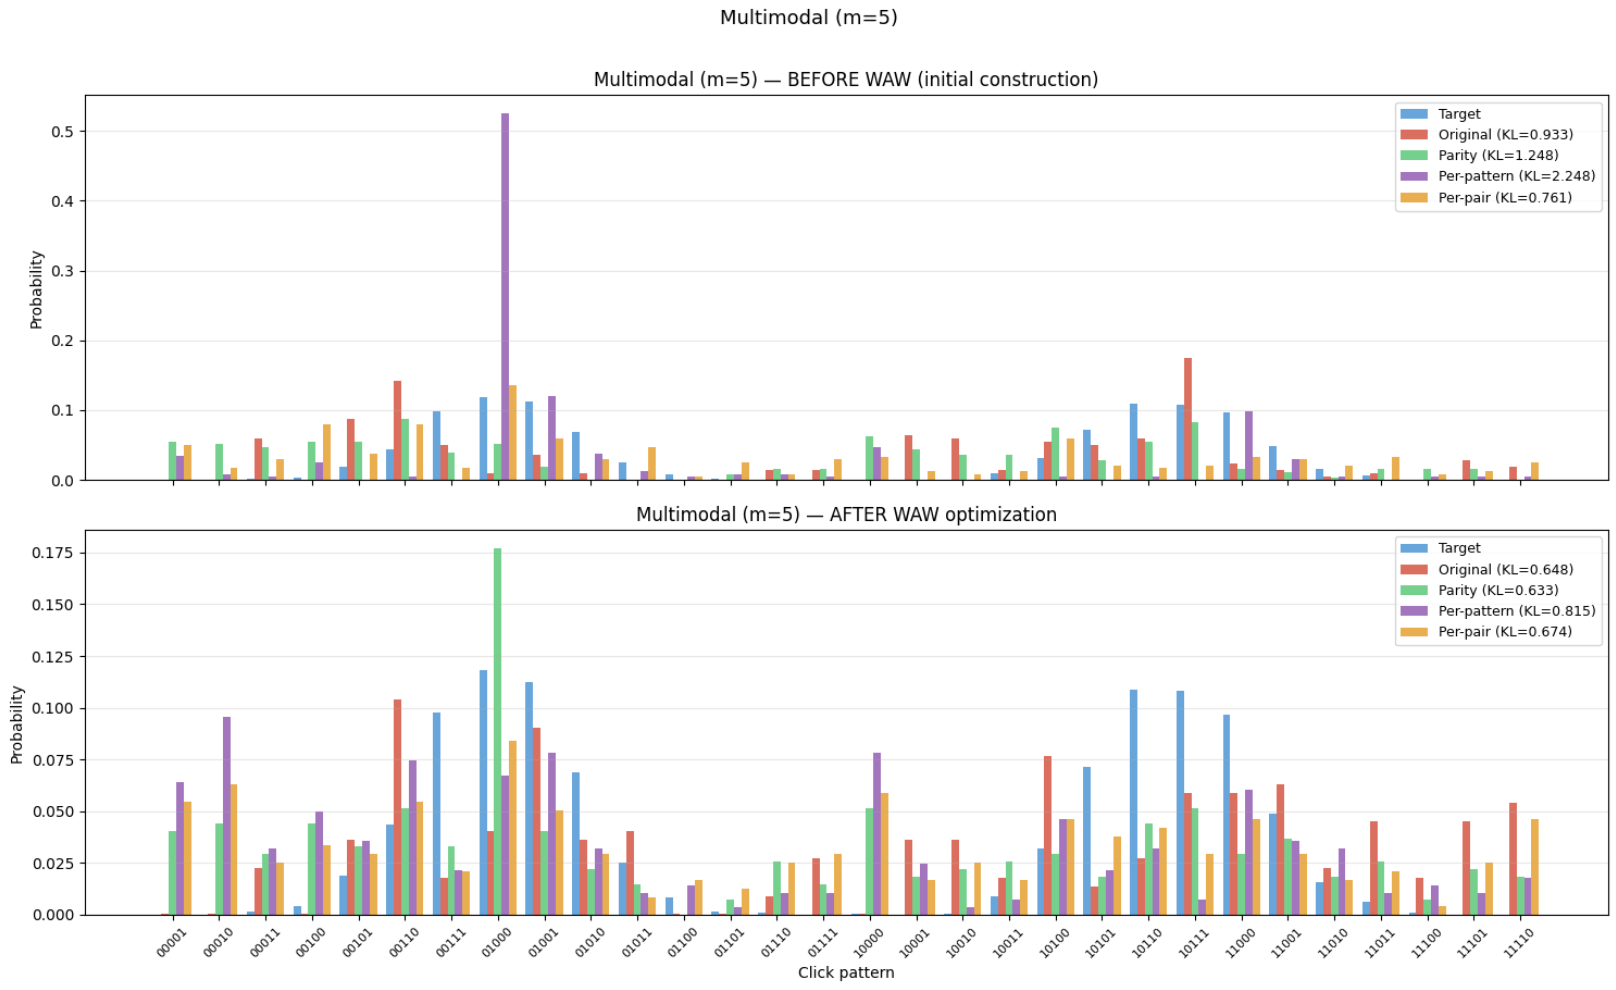
\includegraphics[width=0.84\textwidth]{multimodal_fix.png}\\
{\footnotesize Per-pair (green) vs baseline (red) and per-pattern (purple),
before/after WAW. Baseline over-produces high-click patterns; per-pattern
over-produces low-click ones.}
\end{frame}

\begin{frame}{Encoding matters: Gray code}
Standard binary is \emph{not} Hamming-smooth: adjacent bins can differ in all
$m$ bits ($01111\leftrightarrow10000$). A smooth $p(x)$ becomes non-smooth in
pattern space, which a pairwise (hafnian) model cannot represent.
\[
\text{Reflected Gray code: } g(n)=n\oplus(n\gg1)\quad\Rightarrow\quad
\text{adjacent bins differ by 1 bit.}
\]
\begin{columns}
\begin{column}{0.5\textwidth}
\centering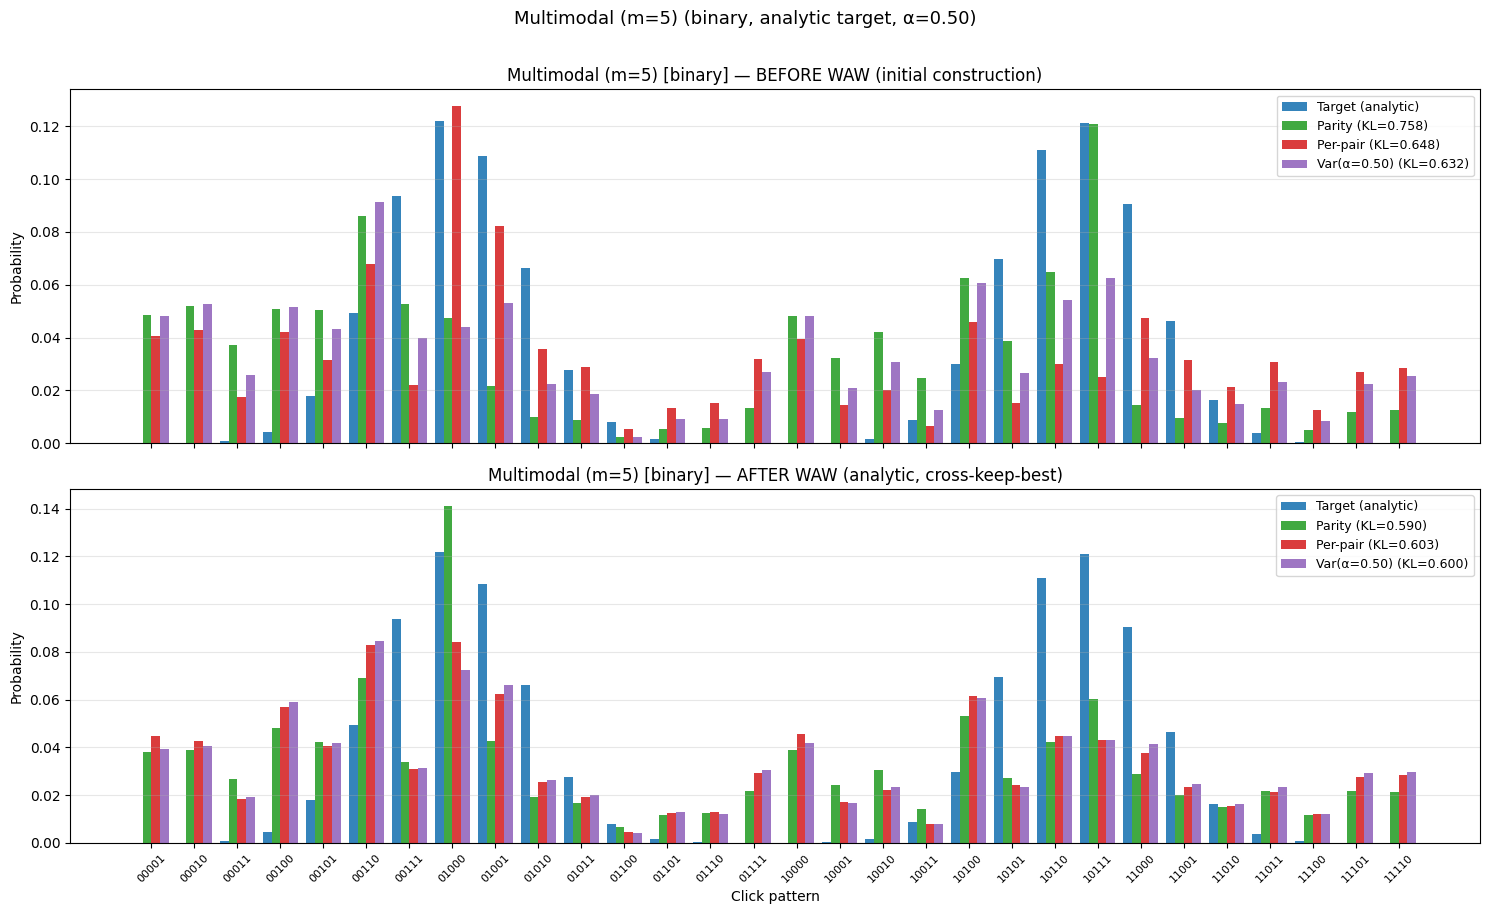
\includegraphics[width=\textwidth]{mmodal_bin.png}\\{\footnotesize binary}
\end{column}
\begin{column}{0.5\textwidth}
\centering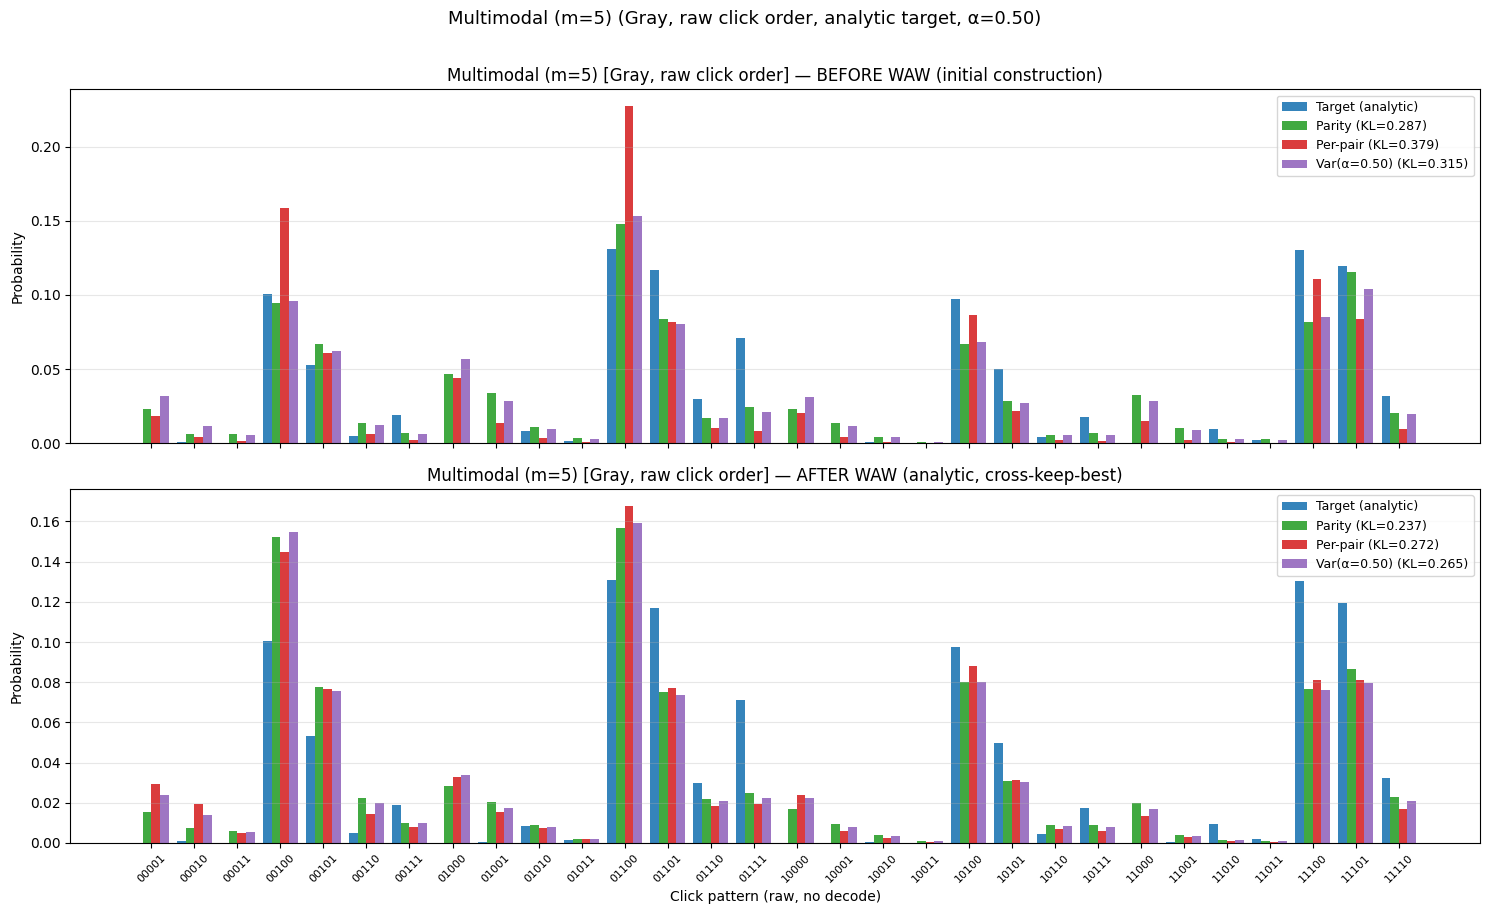
\includegraphics[width=\textwidth]{mmodal_gray.png}\\{\footnotesize Gray}
\end{column}
\end{columns}
\centering{\footnotesize Multimodal: Gray roughly halves the KL.}
\end{frame}

\begin{frame}{Optimisation: two fixes}
\begin{block}{Keep-best}
Baseline WAW: random init, fixed steps, returns \emph{last} iterate $\Rightarrow$
mode collapse on Gray data. Fix: zero init, monitor KL, return the
\emph{best} iterate.
\end{block}
\begin{block}{Analytic KL (and a real bug)}
\texttt{torontonian\_sample\_graph} \alert{silently rescales $A$} at sampling
time $\Rightarrow$ optimised $\neq$ evaluated distribution, KL could
\emph{increase} after training. Fix: minimise the exact analytic KL (torontonian
over all $2^m$ patterns) with keep-best $\Rightarrow$ KL provably non-increasing.
\end{block}
\end{frame}

\begin{frame}{Construction $\times$ encoding: results}
Analytic KL \emph{after} WAW, $m=5$ (best per column in bold):
\begin{center}
\begin{tabular}{lcccccc}
\toprule
 & \multicolumn{2}{c}{Normal} & \multicolumn{2}{c}{Multimodal} & \multicolumn{2}{c}{Log-normal}\\
\cmidrule(lr){2-3}\cmidrule(lr){4-5}\cmidrule(lr){6-7}
Construction & bin & Gray & bin & Gray & bin & Gray\\
\midrule
Baseline   & 0.56 & 0.57 & 0.61 & 0.38 & 0.61 & 0.63\\
Parity     & 0.21 & \textbf{0.13} & 0.59 & \textbf{0.24} & 0.34 & \textbf{0.24}\\
Per-pair   & 0.20 & 0.14 & 0.59 & 0.28 & 0.30 & 0.25\\
Variance   & \textbf{0.19} & 0.13 & \textbf{0.58} & 0.27 & 0.33 & 0.25\\
\bottomrule
\end{tabular}
\end{center}
\begin{itemize}
  \item Smooth targets: the \emph{construction} dominates ($\sim3\times$ KL drop).
  \item Multimodal: the \emph{encoding} dominates (Gray: $0.59\to0.24$).
\end{itemize}
\end{frame}

\begin{frame}{Photon-counting (PNR) readout}
Read $\vn$ directly. For a collision-free $0/1$ pattern
\[
P_{\mathrm{PNR}}(\vs)\ \propto\ \big|\Haf(A[\vs])\big|^2
\quad(\text{support submatrix, no factorial}),
\]
general weight $=|\Haf(A[\vn])|^2/\prod_i n_i!$ --- exactly the clean signal the
threshold heuristics were estimating.
\begin{columns}
\begin{column}{0.5\textwidth}
\centering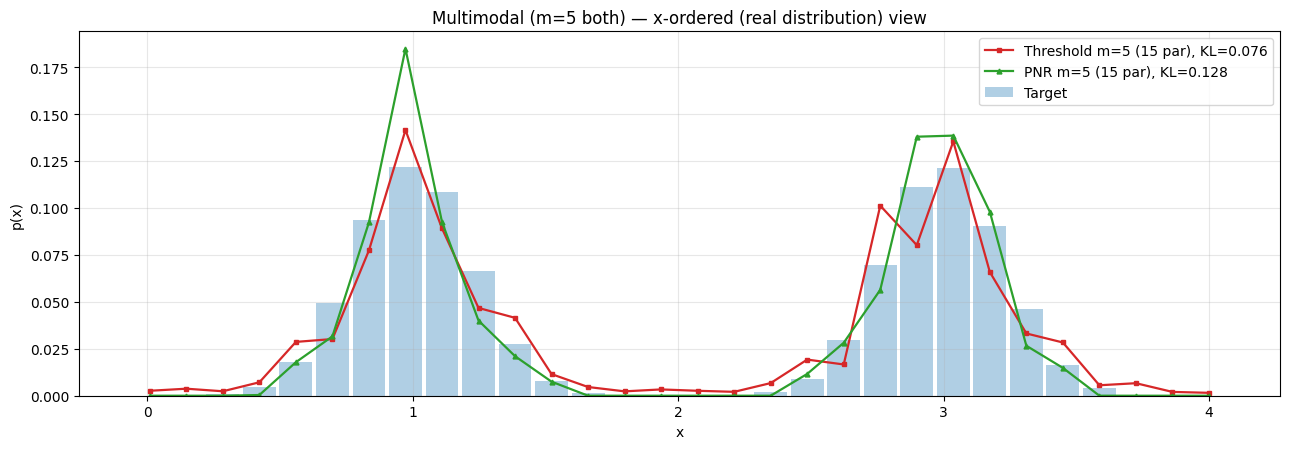
\includegraphics[width=\textwidth]{pnr_mmodal.png}\\{\footnotesize threshold vs PNR}
\end{column}
\begin{column}{0.5\textwidth}
\centering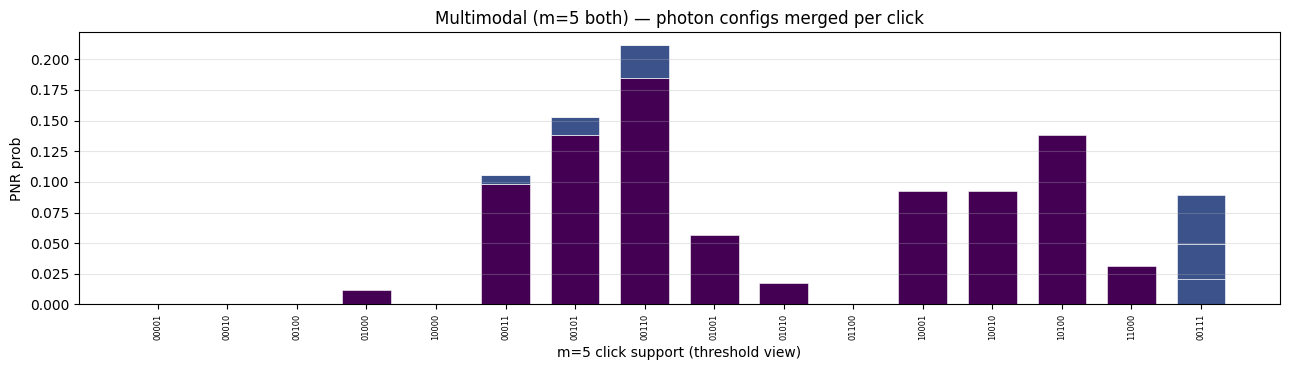
\includegraphics[width=\textwidth]{pnr_merged_mmodal.png}\\{\footnotesize $200,400,\dots\to$ one click}
\end{column}
\end{columns}
\end{frame}

\begin{frame}{PNR: concentration, not a free win}
\begin{columns}
\begin{column}{0.52\textwidth}
\begin{itemize}
  \item At fixed $m$, PNR adds \emph{no} matrix parameters.
  \item Usable outcomes dominated by a steep photon-number magnitude hierarchy
        $\Rightarrow$ needs a probability-matched encoding (else $\KL\!\approx\!3.7$).
  \item PNR family is intrinsically \emph{concentrated}; threshold is \emph{spread}.
\end{itemize}
\end{column}
\begin{column}{0.48\textwidth}
\begin{center}
\begin{tabular}{lcc}
\toprule
$m=6$ & Thresh. & PNR\\
\midrule
fitted entropy & 3.6 & 3.2\\
top-5 mass & 0.27 & 0.43\\
\midrule
KL, Normal (broad) & \textbf{0.05} & 0.53\\
KL, bimodal (conc.) & 0.12 & \textbf{0.08}\\
\bottomrule
\end{tabular}
\end{center}
\end{column}
\end{columns}
\vspace{4pt}
\alert{Match the detector to the target's concentration.}
\end{frame}

\begin{frame}{Selecting the mean photon number $\nmean$}
$\nmean=m/2$ is arbitrary. It is a \emph{concentration knob} (decoupled from the
data by the probability-matched encoding): low $\nmean$ $\to$ concentrated model,
high $\nmean$ $\to$ spread but a stronger central \emph{spike}.
\begin{columns}
\begin{column}{0.6\textwidth}
\centering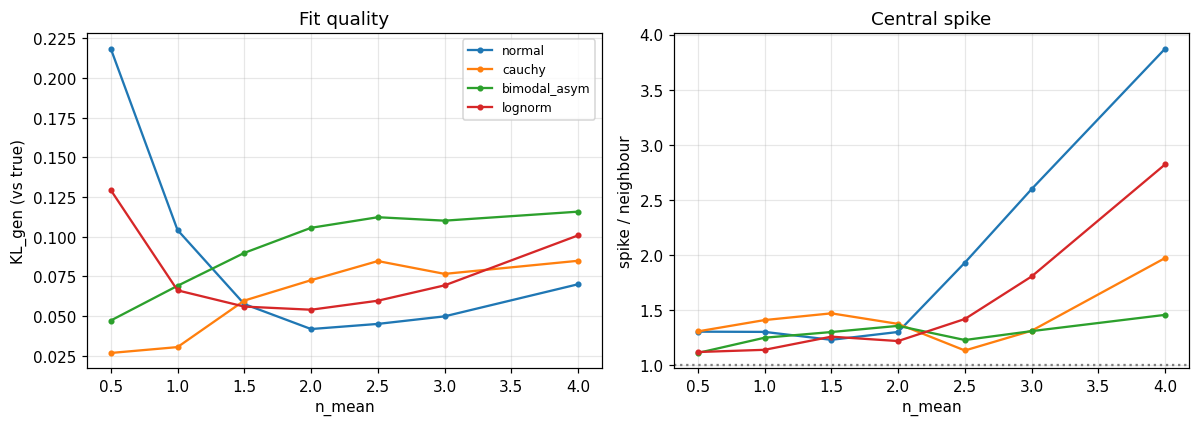
\includegraphics[width=\textwidth]{nmean_selection.png}
\end{column}
\begin{column}{0.4\textwidth}
Select by minimum \emph{empirical} KL:
\begin{itemize}
  \item broad targets $\to \nmean\approx2$;
  \item concentrated $\to \nmean\approx0.5$;
  \item spike grows monotonically with $\nmean$.
\end{itemize}
Always below the default $m/2$.
\end{column}
\end{columns}
\end{frame}

\begin{frame}{Combining threshold + PNR}
Both models map back to the same $x$-bins, so mix them there:
\[
q_{\mathrm{mix}}(x)=w\,q_{\mathrm{thr}}(x)+(1-w)\,q_{\mathrm{PNR}}(x),\qquad
w=\arg\min_w \KL(\hat p\,\|\,q_{\mathrm{mix}}).
\]
Physically realizable (per-shot choice of detector); convex $\Rightarrow$ never
worse than the better single model.
\begin{columns}
\begin{column}{0.62\textwidth}
\centering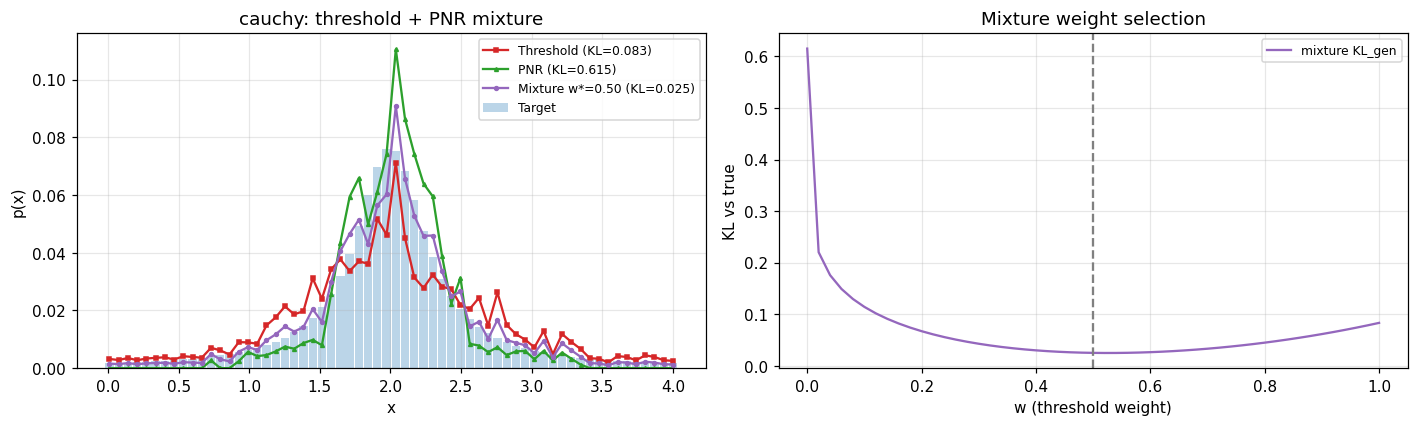
\includegraphics[width=\textwidth]{combine_cauchy.png}
\end{column}
\begin{column}{0.38\textwidth}
\begin{center}
\begin{tabular}{lccc}
\toprule
$m{=}6$ & thr & PNR & mix\\
\midrule
Cauchy & .083 & .615 & \textbf{.025}\\
bimodal & .114 & .077 & \textbf{.039}\\
\bottomrule
\end{tabular}
\end{center}
Wins $2$--$3\times$ on mixed (sharp+broad) structure.
\end{column}
\end{columns}
\end{frame}

\begin{frame}{Scaling study: 9 targets $\times$ $m\in\{4,5,6\}$}
\begin{columns}
\begin{column}{0.46\textwidth}
\centering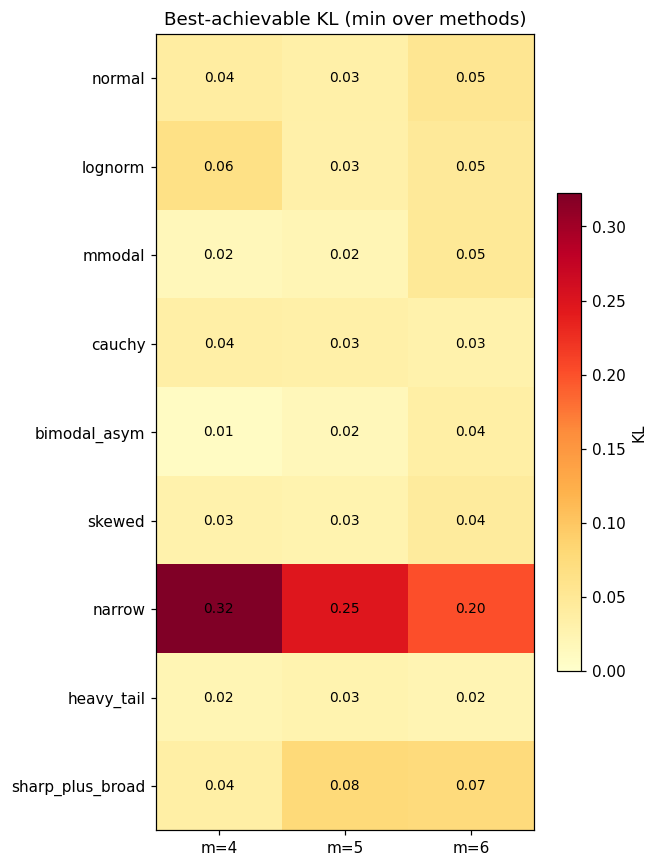
\includegraphics[width=0.85\textwidth]{scaling_heatmap.png}
\end{column}
\begin{column}{0.54\textwidth}
Best-achievable KL (min over methods).
\begin{itemize}
  \item 8/9 targets reach $\KL\lesssim0.08$ at every $m$, incl.\ strongly
        skewed and heavy-tailed.
  \item Extra modes are \emph{used}, not wasted.
  \item One clear outlier: the very \emph{narrow} target (dark row).
\end{itemize}
\end{column}
\end{columns}
\end{frame}

\begin{frame}{Worst case: the concentration ceiling}
\centering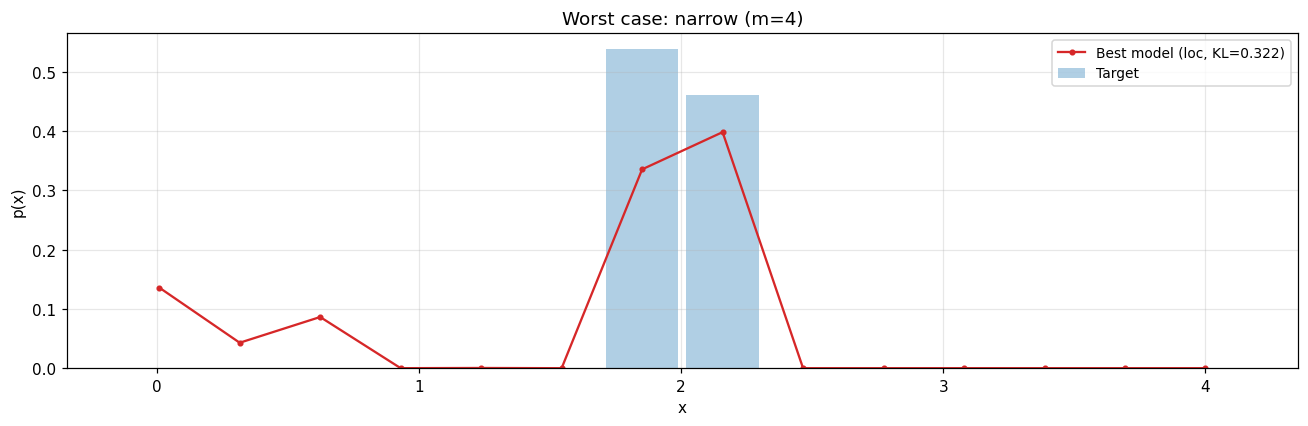
\includegraphics[width=0.9\textwidth]{worstcase_narrow_m4.png}\\
{\footnotesize Very narrow target: model finds the location but leaks $\sim0.13$
onto a distant pattern.}
\begin{itemize}
  \item A GBS click distribution's most-probable pattern cannot carry the
        $\sim0.5$ mass a 2-bin target needs $\Rightarrow$ KL $\approx0.2$--$0.3$.
  \item Mirror image of the multimodal \emph{valley} floor (can't spread) vs
        \emph{concentration ceiling} (can't pile up). Eases with larger $m$.
\end{itemize}
\end{frame}

\begin{frame}{Honesty checks: encoding from samples, and a mixture bound}
\begin{block}{Sample-only encoding}
The probability-matched encoding uses the \emph{empirical} histogram $\hat p$
(not the true target). $\KL_{\mathrm{train}}\!\approx\!\KL_{\mathrm{gen}}$ and it
matches the oracle to within $\sim0.01$ KL --- not a hidden cheat.
\end{block}
\begin{block}{Local (per-bin) mixture: no robust gain}
$w(x)=\sigma(a+b\,r(x))$, $r=$ local peakiness. Matches the global mixture, not
better. The per-bin \emph{convex-hull bound} shows headroom exists, but a simple
gate cannot realise it and richer fitting overfits. Global mixture stays the
recommendation.
\end{block}
\end{frame}

\begin{frame}{Summary of results}
\begin{itemize}
  \item \textbf{Bias:} parity/factorial structure $\Rightarrow$ parity \& per-pair
        constructions; variance (click-count) matching for the photon budget.
  \item \textbf{Encoding:} Gray code is decisive for multimodal ($\sim2\times$).
  \item \textbf{Optimisation:} analytic keep-best makes KL monotone; fixed a
        silent-rescale bug.
  \item \textbf{Readout:} threshold (spread) vs PNR (concentrated); their convex
        \emph{mixture} wins $2$--$3\times$ on mixed-structure targets.
  \item \textbf{$\nmean$:} a concentration hyperparameter to be selected, not fixed.
  \item Net: $\sim3\times$ KL reduction on smooth targets, $\sim2.5\times$ on
        multimodal; 8/9 targets $\KL\lesssim0.08$.
\end{itemize}
\end{frame}

\begin{frame}{Limits, and what this is (not)}
\begin{block}{Honest scope}
For a 1-D density a histogram / inverse-CDF sampler is exact --- GBS does not
compete as a \emph{sampler}, and these sizes are classically simulable (no
advantage). The value is a \textbf{characterisation of GBS as a trainable
model} + reusable evaluation methodology.
\end{block}
\begin{block}{Three structural limits}
\begin{enumerate}
  \item Multimodal \emph{valley} — expressivity floor of one Gaussian state.
  \item \emph{Concentration ceiling} — narrow peaks (worst case).
  \item Per-bin mixture headroom not realised by a simple gate.
\end{enumerate}
\end{block}
\textbf{Outlook:} displacement / GBS mixtures (attack floor \emph{and} ceiling);
pivot to GBS-native targets (graphs) where the adjacency matrix is the natural
object.
\end{frame}

\begin{frame}{References}
\footnotesize
\begin{thebibliography}{9}
\bibitem{banchi2020} L.~Banchi, N.~Quesada, J.~M.~Arrazola,
\emph{Training Gaussian Boson Sampling Distributions}, PRA \textbf{102}, 012417 (2020).
\bibitem{quesada2018} N.~Quesada, J.~M.~Arrazola, N.~Killoran,
\emph{Gaussian boson sampling using threshold detectors}, PRL \textbf{121}, 110503 (2018).
\bibitem{hamilton2017} C.~S.~Hamilton \emph{et al.},
\emph{Gaussian Boson Sampling}, PRL \textbf{119}, 170501 (2017).
\bibitem{kruse2019} R.~Kruse \emph{et al.},
\emph{Detailed study of Gaussian boson sampling}, PRA \textbf{100}, 032326 (2019).
\end{thebibliography}
\end{frame}

\begin{frame}
\centering\Large Thank you --- questions?
\end{frame}

% ======================================================================
\appendix
\section*{Appendix}
% ======================================================================

\begin{frame}{Appendix: the physical device}
Three stages behind the matrix $A$:
\begin{enumerate}
  \item \textbf{Sources.} Each mode in single-mode squeezed vacuum
        $\ket{\xi_j}=S(\xi_j)\ket0$,
        $S(\xi)=\exp\!\big[\tfrac12(\xi^\ast a^2-\xi a^{\dagger2})\big]$,
        $\xi_j=r_je^{i\phi_j}$.
  \item \textbf{Interferometer.} Passive network $U\in U(m)$:
        $a_i^\dagger\mapsto\sum_jU_{ij}a_j^\dagger$ $\Rightarrow$
        $A=U\,\mathrm{diag}(\tanh r_j)\,U^{\mathsf T}$.
  \item \textbf{Detection.} PNR or threshold detectors.
\end{enumerate}
\begin{block}{Squeezed vacuum has only even photon numbers}
\[
\ket{\xi}=(\cosh r)^{-1/2}\sum_{n\ge0}
\frac{\sqrt{(2n)!}}{2^n\,n!}\,(-e^{i\phi}\tanh r)^n\,\ket{2n}.
\]
$\Rightarrow$ even total photon number (parity) --- the root of the Part~II bias.
\end{block}
\end{frame}

\begin{frame}{Appendix: Gaussian-state formalism and the two $A$'s}
A Gaussian state is fixed by its mean $\bm\mu$ and covariance $V$
($\bm\mu=0$ for standard GBS). The $2m\times2m$ \textbf{kernel matrix}
$\mathbf A$ (bold) comes from the covariance:
\[
\mathbf A=X\big(I-(V+\tfrac12 I)^{-1}\big),\qquad
X=\begin{pmatrix}0&I\\I&0\end{pmatrix},\qquad
Z=\sqrt{\det(I-X\mathbf A)} .
\]
\begin{itemize}
  \item General outcome law: $P(\vn)=\tfrac1Z\,\Haf(\mathbf A_{\vn\oplus\vn})/\prod_i n_i!$.
  \item For a \emph{pure} state $\mathbf A=A\oplus A^\ast$ with the $m\times m$
        symmetric block $A$ (plain) used on the main slides; it reduces to
        $P_A(\vn)=\tfrac1Z\,|\Haf(A_{\vn})|^2/\prod_i n_i!$.
  \item Per-mode photon number (WAW gradient):
        $\langle n_k\rangle=V_{kk}+V_{k+m,k+m}-\tfrac12$.
\end{itemize}
\end{frame}

\begin{frame}{Appendix: displacement (breaking parity)}
Replace squeezed vacuum by \emph{displaced} squeezed vacuum $D(\alpha)S(\xi)\ket0$,
$\bm\mu\neq0$. Then even/odd photon numbers both appear (parity lifted), and
probabilities use the \textbf{loop} hafnian / \textbf{loop} torontonian:
\[
P(\vs)=P_{\mathrm{vac}}\,\mathrm{ltor}\!\big(O_{\vs},\bm\gamma_{\vs}\big),\qquad
\bm\gamma=(\sigma_Q^{-1}\bm\alpha)^\ast .
\]
Adds $2m$ parameters $\bm\mu\in\mathbb R^{2m}$; a scalable surrogate trains WAW
first, then one scalar displacement by binary search on the odd-parity fraction.
\end{frame}

\begin{frame}{Appendix: the analytic KL gradient (derivation sketch)}
From $P_{A,W}(\vn)=\tfrac1Z|\Haf(A_{\vn})|^2\prod_i w_i^{n_i}/n_i!$ and
$\Haf$ independent of $\bm w$:
\[
\partial_{w_k}\ln P_{A,W}=\frac{n_k-\langle n_k\rangle}{w_k}
\ \Rightarrow\
\partial_{\bm\theta}C=\sum_k\big(\langle n_k\rangle_{\mathrm{GBS}}-\langle n_k\rangle_{\mathrm{data}}\big)f^{(k)} .
\]
With $F_{\mathrm{data}}=\sum_k\langle n_k\rangle_{\mathrm{data}}f^{(k)}$ precomputed,
each step needs only the $m$ model means $\langle n_k\rangle_{\mathrm{GBS}}$
($O(m)$ from $V$) --- classical and fast even when sampling is hard.
\end{frame}

\end{document}
